\chapter{Paper Pinch} \label{chap:pidPinch}

\section{Case Description}
The paper pinch co-model illustrates a device for
manipulating paper (e.g., in a printer) and includes several
different types of fault modelling. A pair of rollers sit one
above the other and a motor is capable of rotating the
bottom-mounted one. The top roller is spring loaded to produce a
light downward pressure at all times. Rotating the bottom roller
allows the pair to `pinch' a sheet of paper and pass it between
the two rollers, thus moving it through the printer. An overview
of the rollers and motor and how they are connected can be seen
in Fig~\ref{fig:paperPinch}.

\begin{figure}[!ht] \centering
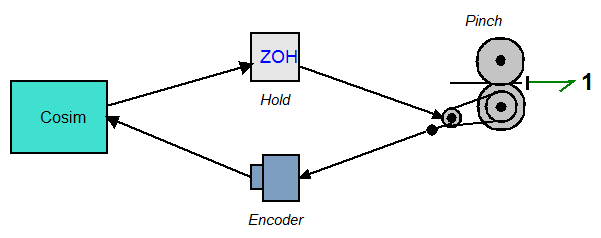
\includegraphics[width=0.7\textwidth]{pidPinch/pidPinch.png}
\caption{Diagram of a single pair of rollers in a printer
("Pinch"), the cosim Controller, an output line between
controller and pinch (with a zero-order hold) and an encoder to
feed data back to the Controller.} \label{fig:paperPinch}
\end{figure}

A real printer might typically have many sets of `pinches' to
manipulate the paper from an input tray through the printing
process to the output tray. This often involves moving the paper
in S-curves as well as in a simple linear direction. There is a
requirement that the pinches in the system move paper at a
synchronised speed. If one pinch feeds the paper too quickly or
too slowly to its neighbours then the paper will fold and bunch
up between the sets of pinches, or will be torn, and result in a
paper jam. Alternatively the paper may become skewed,
resulting in suboptimal print quality.

The main purpose of this co-model is to simulate some different
types of fault handling. The co-model allows the modelling of
two types of faults and two fault tolerant techniques.

\section{External Links}
The model was described in \cite{Pierce&11}.  This paper demonstrated
the modelling and simulation of errors and fault tolerance mechanisms
for embedded systems.

\section{Contract} The contract contains four shared state
variables of type \keyw{real}. One of these is responsible for
signalling power to the actuator \texttt{pwm}. This increases or
decreases the speed of the roller to control movement of the
paper through the pinch. Three more shared state variables are
used to read the current speed of the rollers, delivered by
three separate encoders: \texttt{enc1}, \texttt{enc2} and
\texttt{enc3}. %\begin{itemize} %\item Monitored variables
%\item Controlled variables %\item Shared design parameters
%\end{itemize}

\section{Discrete-event} The DE model implements a basic Decorator
pattern (as described by Gamma \emph{et al} \cite{gamma}), consisting
of the \texttt{Controller} which has the main thread of control, as
well as an \texttt{ISensorInt} abstract class to monitor the readings
from the pinch and an \texttt{IActuatorPWM} abstract class to produce
a power signal to the actuators. In the model \texttt{Encoder} is
provided as a possible implementation of the abstract
\texttt{ISensorInt}, and \texttt{PWM} is provided as a possible
implementation of the abstract \texttt{IActuatorPWM}.

The paper pinch model simulates several types of faults, and also
incorporates several methods for fault tolerance (see
Section~\ref{sec:CTpinch} for details of faults which are
injected). Firstly, the \texttt{Controller} is capable of implementing
a voting system, which helps to detect cases where a single encoder
has produced an incorrect value. This functionality is implemented in
the \texttt{Voter} class, which is an alternative implementation of
\texttt{ISensorInt}.  \texttt{Voter} considers inputs from multiple
sensors and translates this into a single value.

A further aspect of fault management is implemented in the
\texttt{SafetyKernel} class, which is an alternative implementation of
\texttt{IActuatorPWM}. \texttt{SafetyKernel} intercepts the
controller's output to the power line and caps the signal to some
absolute value.  This prevents sudden large increases or decreases in
power delivered to the actuator; if a mistake has been made and the
\texttt{Controller} produces an inappropriate power output to the
actuator, then this behaviour will curb the severity of the fault.

\section{Continuous-time} \label{sec:CTpinch}
The CT model includes a controller block (\texttt{Cosim}) which
handles the interface with the DE model. The controller produces a
power signal to an actuator, which then rotates the bottom roller in
the pinch device. Sensors detect the actual rotational speed achieved
by the pinch and several encoders feed this information back to the
controller.  The input to the encoder is the speed of some shaft in
revolutions per second and the output is a count indicating the number
of rotations.

The purpose of this co-model is to simulate fault handling and so the
co-model includes three encoders, to allow the model to simulate
different types of faults. Each encoder includes a fault block that
can intercept the input to the encoder and inject a possible
fault. One of the three encoders is fault-free, one produces
occasional bit-flips (sudden, large-value errors in the reading) and
the final encoder produces a `drift' error (low-value, cumulative,
gradual errors in the reading).  The fault blocks can be individually
triggered to inject a fault.

\section{Usage of fault tolerant features} The primary purpose of this model is to
simulate different types of fault and fault tolerance, and so one
obvious scenario is to test the fault handling.  As previously
described in Section \ref{sec:CTpinch}, there are three encoders, each
with a fault block.  By default, one fault block in this model is set
to produce a bit-flip error (characterised by a sudden large error in
the value read in); one is set to produce a `drift' type of error
(characterised by small, gradual errors); and one fault block is
configured to produce no error at all.  Running a simulation with the
default configuration will show output from all three encoders
alongside their respective fault blocks; a change in the signal for a
fault block indicates that it has activated and injected a fault into
the model.  There will be subsequent changes in other readings as the
model detects and copes with the change.  For example, when a bit-flip
fault is triggered, the output from \texttt{Encoder1} can be seen to
change value suddenly. If the model is employing the fault tolerant
\texttt{Voter} and \texttt{SafetyKernel} implementations of the
\texttt{ISensorInt} and \texttt{IActuatorPWM} classes, the
\texttt{Voter} class can cope with the bit flip by considering the
values of all three encoders and deciding that because the reading
from \texttt{Encoder1} does not correspond with the others it is a
fault and should be ignored; as a result the output value from the
\texttt{Controller} does not change.

\begin{figure}[!ht] \centering
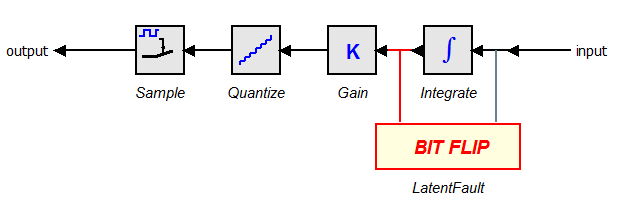
\includegraphics[width=0.7\textwidth]{pidPinch/pidPinchFaultBlock.png}
\caption{Diagram of the blocks inside an encoder for the paper pinch
  co-model, showing a fault block intercepting the input value.}
\label{fig:paperPinchFaultBlock}
\end{figure}

A good next step would be to configure the fault blocks.  Any of the
fault blocks can be set to produce a bit-flip fault, a bit-drift
fault, or no fault at all.  To to this, open the CT model in 20-sim
and double click on an encoder block to open it up.  Figure
\ref{fig:paperPinchFaultBlock} shows an encoder with a fault block
attached; the fault block, when triggered, tampers with the input
signal and produces an erroneous output.  To configure the fault
block, right-click on it and select "Edit Implementation".  This
produces a menu with "bitflip", "drift" and "nofault" as options.
Using this method, it's possible to change the type of error that is
produced for different encoders.  It's also possible to configure the
time in the simulation at which the fault block is triggered to
produce a fault.  To do this, right-click on the fault block and
select "Parameters" (click "yes" if 20-sim asks if it should check the
model first).  This produces a dialog box where parameters for the
fault block are set; changing the value for the "fault\_time"
parameter will change the time when the fault-block activates and
injects a fault during the simulation.  We recommend experimenting
with changing the types of error on each encoder, and changing the
times when faults are triggered, and then running the simulation to
examine how the model copes with different types of fault: i.e., how
quickly it can detect them and take some corrective action.


